\chapter{Eksperymenty dla schematu licencyjnego Duolingo Super}
\label{chap:experiments}
\section{Środowisko i metodologia}

Eksperymenty wykonano na komputerze z procesorem Intel Core i5-14600KF (12 rdzeni ograniczone przez konfigurację Wyniki potwierdzają również znaczenie struktury grafu. W przypadku grafów losowych i małoświatowych uzyskuje się wyniki zbliżone do solvera ILP, natomiast grafy bezskalowe generują wyższe koszty. Rysunek~\ref{fig:duo-real-size} ilustruje, że przeszukiwanie tabu utrzymuje niskie koszty na węzeł także przy rosnącej liczbie wierzchołków, a czasy działania rosną umiarkowanie.SL2, taktowanie 3.49~GHz) oraz 16~GB pamięci RAM. System operacyjny stanowił Ubuntu~24.04~LTS uruchomiony w środowisku WSL2. Implementacja algorytmów powstała w języku Python~3.13; wykorzystano biblioteki NumPy, NetworkX, a także PuLP jako interfejs do algorytmów ILP. Każdy pomiar obejmował wyłącznie czas obliczeń, pomijając koszt przygotowania instancji oraz operacje wejścia/wyjścia.

Środowisko badawcze udostępniono jako zbiór skryptów w języku Python. Osobne moduły obsługują benchmark statyczny, symulacje dynamiczne oraz scenariusze rozszerzeń, a uproszczone polecenia w interfejsie wiersza poleceń umożliwiają uruchamianie pojedynczych algorytmów w trybie diagnostycznym. Taki podział umożliwia równoległe prowadzenie rozległych serii eksperymentów i sprawną weryfikację jakości poszczególnych metod.

Analiza objęła dwa zestawy danych: syntetyczne grafy losowe, bezskalowe oraz małoświatowe o liczebności od 50 do 450 wierzchołków, a także grafy ego z serwisu Facebook o liczebności od 53 do 1035 wierzchołków. Dla każdej instancji uruchamiano wszystkie algorytmy z limitem czasu 60 s, a przekroczenie tego limitu klasyfikowano jako przekroczenie limitu czasu i wyłączano z dalszych obliczeń. W przypadku grafów syntetycznych odnotowano w sumie 10 przekroczeń limitu czasu dla algorytmu mrówkowego oraz algorytmu ILP, natomiast na grafach rzeczywistych odpowiednio 8, 18 i 6 przypadków dla algorytmu mrówkowego, algorytmu ILP oraz przeszukiwania tabu. Wszystkie pozostałe uruchomienia zakończyły się sukcesem.

W przypadku grafów syntetycznych dla każdego rozmiaru generowano trzy niezależne instancje, a następnie wykonywano po dwa uruchomienia algorytmów na każdej z nich. Analiza sieci ego Facebooka obejmowała po jednym grafie na rozmiar oraz dwa powtórzenia dla każdej pary (graf, algorytm), co pozwoliło oszacować zmienność wyników przy zachowaniu określonego budżetu obliczeniowego. W każdej próbie zapisano całkowity koszt licencji, czas wykonania oraz średni koszt licencji przypadający na jednego użytkownika (wierzchołek). Wyniki agregowano jako wartości średnie. Istotność różnic między algorytmami oceniono przy użyciu testów Friedmana, gdzie $\chi^2_F$ to wartość statystyki testu Friedmana oraz $p$ to poziom istotności, a następnie następujących po nich porównań post-hoc metodą Nemenyi'ego. Na syntetycznym benchmarku otrzymano statystyki $\chi^2_F = 577.93$ dla czasu oraz $\chi^2_F = 518.01$ dla kosztu na węzeł ($p < 10^{-100}$ w obu przypadkach), co uzasadnia szczegółowe porównania par algorytmów.

Dodatkowo, w celu ułatwienia porównań między różnymi typami licencji, ceny każdej z licencji zostały znormalizowane. Cena licencji indywidualnej została ustalona na poziomie 1, a ceny licencji grupowych przeskalowano zgodnie z ich pierwotnym stosunkiem do ceny licencji indywidualnej. Dzięki temu możliwe było bardziej przejrzyste porównanie kosztów między różnymi strategiami licencjonowania, niezależnie od ich bezwzględnych wartości.

\subsection{Przykład uruchomienia aplikacji i interpretacja wyników}

Aby uruchomić eksperymenty, należy skorzystać z polecenia \texttt{make pipeline}, które uruchamia główny potok eksperymentalny:
\begin{verbatim}
UV_CACHE_DIR=.cache/uv PYTHONPATH=src uv run python -m glopt.experiments.pipeline
\end{verbatim}

Na rysunku~\ref{fig:cli-content} przedstawiono przykładowy przebieg uruchomienia aplikacji z poziomu terminala.

\begin{figure}[H]
  \centering
  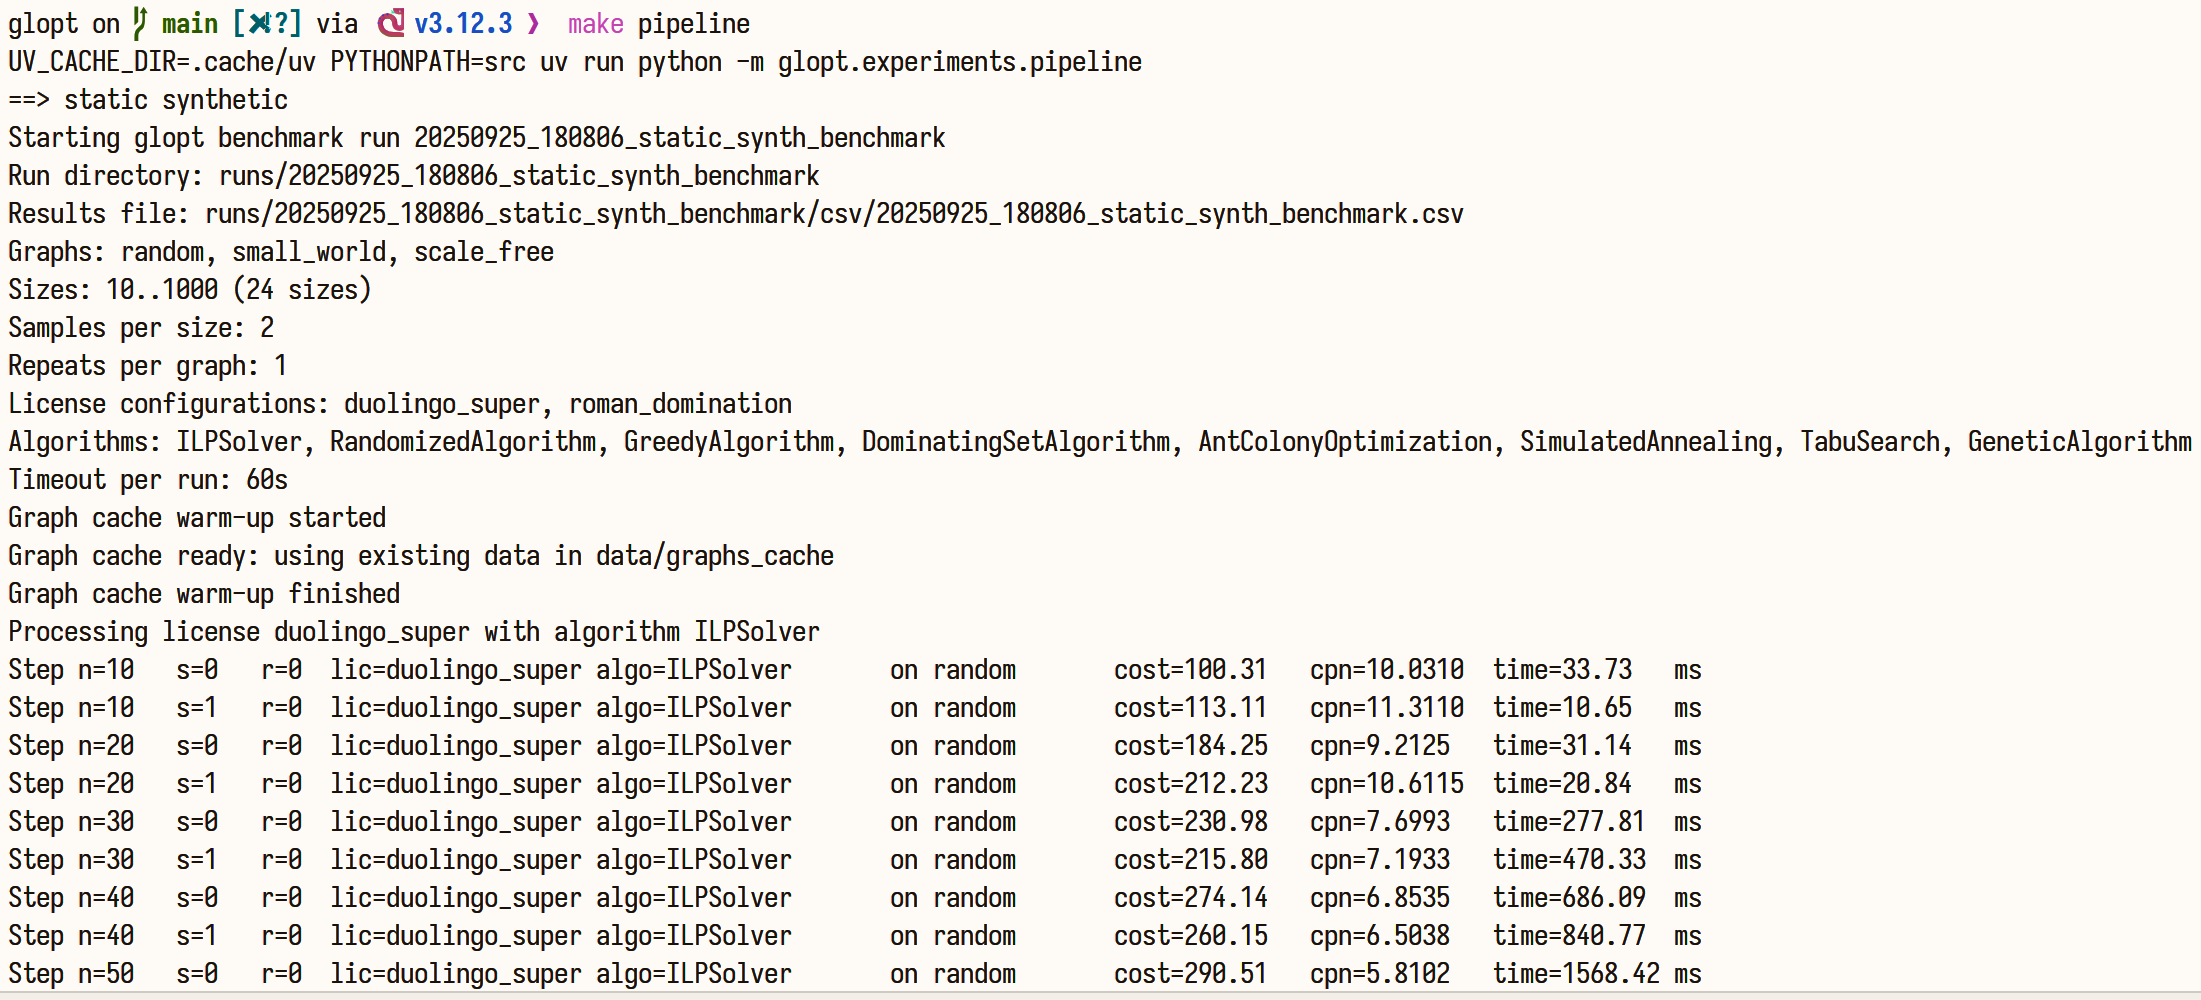
\includegraphics[width=0.95\linewidth]{assets/cli-content.png}
  \caption{Przykładowy przebieg uruchomienia potoku eksperymentalnego z Makefile.}
  \label{fig:cli-content}
\end{figure}

Na początku wyświetlane są informacje o wybranych parametrach uruchomienia, takich jak typ potoku, konfiguracje licencji, lista algorytmów oraz limity czasowe. Następnie rozpoczyna się proces przygotowania grafów. Tworzona jest pamięć podręczna grafów (cache), która umożliwia wielokrotne wykorzystanie tych samych instancji grafów między różnymi algorytmami i konfiguracjami licencji. Eliminuje to konieczność ponownego generowania grafów dla każdej próby, co istotnie skraca czas obliczeń, zwłaszcza dla dużych instancji.

Po przygotowaniu grafów wyświetlane są szczegóły dotyczące liczby rozmiarów, próbek i powtórzeń dla każdej instancji. Następnie dla każdej kombinacji licencji i algorytmu prezentowane są postępy obliczeń. Każda iteracja prezentuje podstawowe statystyki, takie jak rozmiar grafu, koszt rozwiązania, koszt na węzeł oraz czas wykonania. Umożliwia to bieżące monitorowanie przebiegu eksperymentu i szybkie wykrywanie ewentualnych anomalii.

\section{Duolingo Super na grafach syntetycznych}

\subsection{Statystyki zbiorcze}
Tabela~\ref{tab:duo-synth-summary} zestawia średnie wartości kosztu licencji na wierzchołek oraz czasu dla schematu licencyjnego Duolingo Super. Aby zapewnić porównywalność wyników, analizy statystyczne i wizualizacje oparto na podzbiorze instancji, dla których wszystkie algorytmy zakończyły działanie przed upływem limitu czasu; w praktyce oznacza to przycięcie rozmiarów grafów do zakresu wspólnego dla solvera ILP i algorytmu mrówkowego, które najczęściej przekraczały limit. Solver ILP pozostaje najlepszym punktem odniesienia jakościowego (średni koszt na węzeł 0{,}445), lecz ma zastosowanie jedynie dla mniejszych instancji. Liczba przekroczeń limitu czasu jest taka sama jak w algorytmie mrówkowym. Wśród metaheurystyk najniższy koszt na węzeł osiąga właśnie algorytm mrówkowy (0{,}506), natomiast przeszukiwanie tabu zapewnia najlepszy kompromis kosztu na węzeł i czasu w grupie metod przybliżonych. Algorytm zachłanny i algorytm losowy charakteryzują się czasem działania rzędu milisekund, ale tylko pierwszy z nich utrzymuje akceptowalny koszt na węzeł (0{,}548), podczas gdy algorytm losowy generuje rozwiązania o istotnie wyższym koszcie na węzeł.

\begin{table}[H]
  \centering
  \caption{Średnie wartości kosztu na węzeł i czasu dla schematu licencyjnego Duolingo Super na grafach syntetycznych.}
  \label{tab:duo-synth-summary}
  \begin{tabular}{lrrr}
    \toprule
    \textbf{Algorytm}     & \textbf{Średni koszt/węzeł} & \textbf{Średni koszt} & \textbf{Średni czas [s]} \\
    \midrule
    Algorytm ILP          & 0.445                       & 73.83                 & 2.492                    \\
    Algorytm mrówkowy     & 0.506                       & 83.58                 & 5.124                    \\
    Przeszukiwanie tabu   & 0.500                       & 117.80                & 3.298                    \\
    Algorytm genetyczny   & 0.515                       & 118.36                & 1.222                    \\
    Wyżarzanie symulowane & 0.531                       & 120.90                & 0.975                    \\
    Zbiór dominujący      & 0.542                       & 119.97                & 0.017                    \\
    Algorytm zachłanny    & 0.548                       & 121.94                & 0.001                    \\
    Algorytm losowy       & 0.799                       & 179.90                & 0.001                    \\
    \bottomrule
  \end{tabular}
\end{table}


\subsection{Porównanie algorytmów na grafach syntetycznych}

Rysunki~\ref{fig:duo-synth-cost-random}--\ref{fig:duo-synth-cost-small-world} ilustrują, że algorytmy dla schematu licencyjnego Duolingo Super osiągają wyniki porównywalne z algorytmem ILP w przypadku grafów losowych i małoświatowych. Natomiast w przypadku grafów bezskalowych wyniki są zauważalnie gorsze.


\begin{figure}[H]
  \centering
  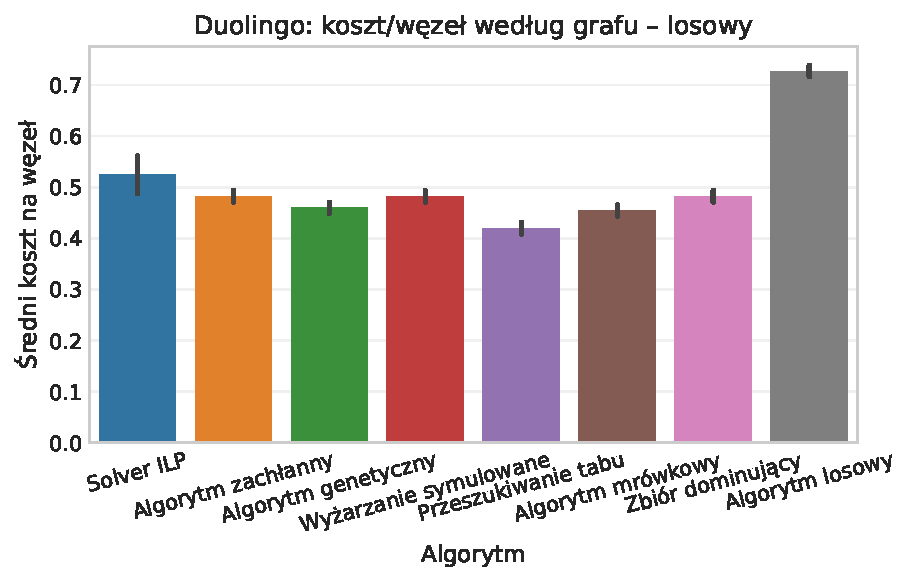
\includegraphics[width=0.65\linewidth]{assets/figures/benchmark/synthetic/duolingo_cost_per_node_by_graph_random.pdf}
  \caption{Koszt na węzeł w zależności od struktury grafu losowego.}
  \label{fig:duo-synth-cost-random}
\end{figure}

\begin{figure}[H]
  \centering
  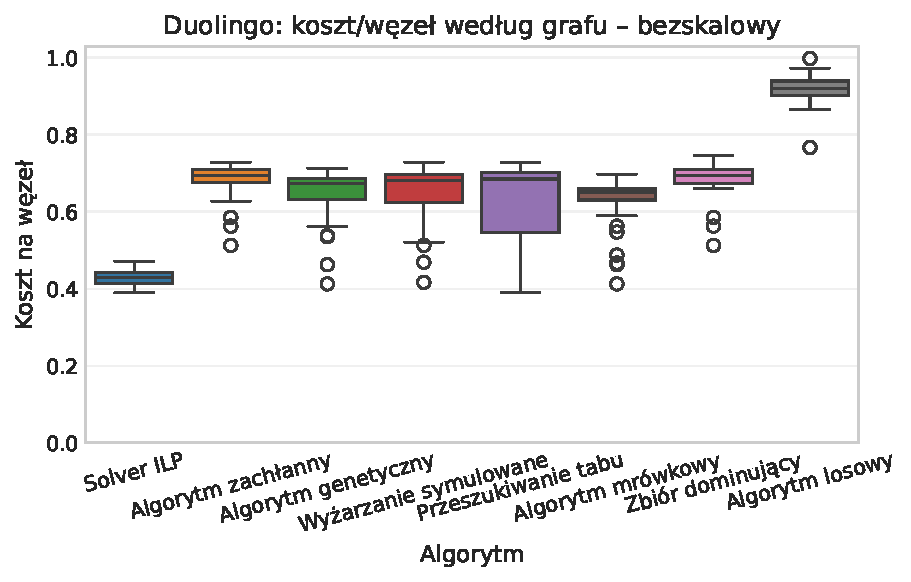
\includegraphics[width=0.65\linewidth]{assets/figures/benchmark/synthetic/duolingo_cost_per_node_by_graph_scale_free.pdf}
  \caption{Koszt na węzeł w zależności od struktury grafu bezskalowego.}
  \label{fig:duo-synth-cost-scale-free}
\end{figure}

\begin{figure}[H]
  \centering
  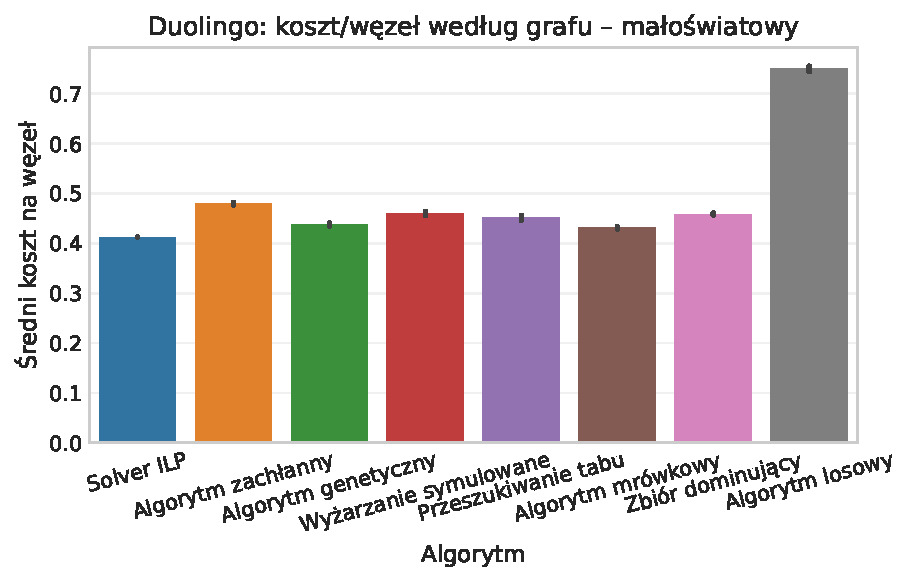
\includegraphics[width=0.65\linewidth]{assets/figures/benchmark/synthetic/duolingo_cost_per_node_by_graph_small_world.pdf}
  \caption{Koszt na węzeł w zależności od struktury grafu małoświatowego.}
  \label{fig:duo-synth-cost-small-world}
\end{figure}

Podobne obserwacje dotyczą czasów wykonania, jak ilustrują rysunki~\ref{fig:duo-synth-time-random}--\ref{fig:duo-synth-time-small-world}. Czasy działania algorytmów są zbliżone dla różnych typów grafów, z wyjątkiem algorytmu ILP, który średnio osiąga krótszy czas wykonania na grafach bezskalowych, oraz przeszukiwania tabu, które działa na nich dłużej. Pozostałe algorytmy wykazują porównywalne czasy działania niezależnie od struktury grafu. Tabela~\ref{tab:duo-synth-summary-times} podsumowuje średnie czasów i kosztów na węzeł dla różnych typów grafów.

\begin{figure}[H]
  \centering
  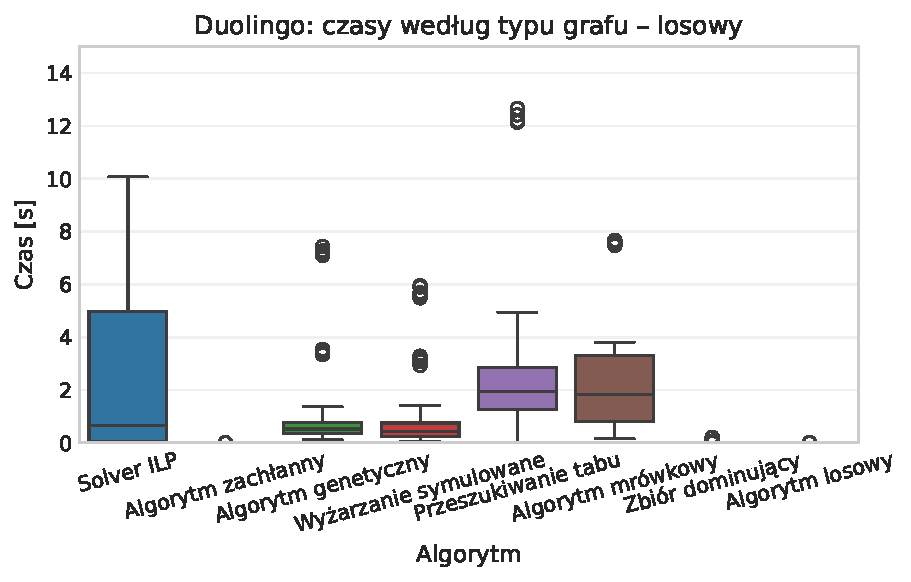
\includegraphics[width=0.65\linewidth]{assets/figures/benchmark/synthetic/duolingo_time_by_graph_random.pdf}
  \caption{Czas wykonania w zależności od struktury grafu losowego.}
  \label{fig:duo-synth-time-random}
\end{figure}

\begin{figure}[H]
  \centering
  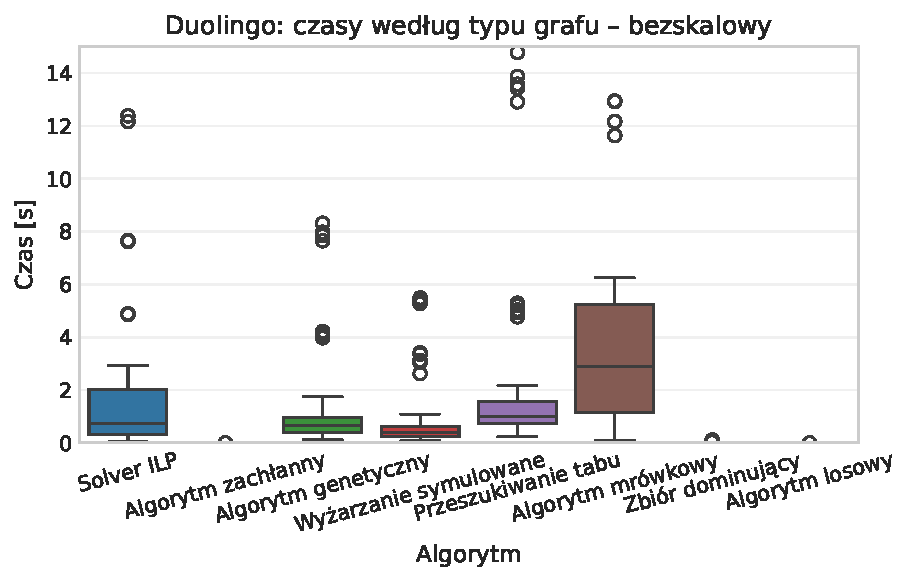
\includegraphics[width=0.65\linewidth]{assets/figures/benchmark/synthetic/duolingo_time_by_graph_scale_free.pdf}
  \caption{Czas wykonania w zależności od struktury grafu bezskalowego.}
  \label{fig:duo-synth-time-scale-free}
\end{figure}

\begin{figure}[H]
  \centering
  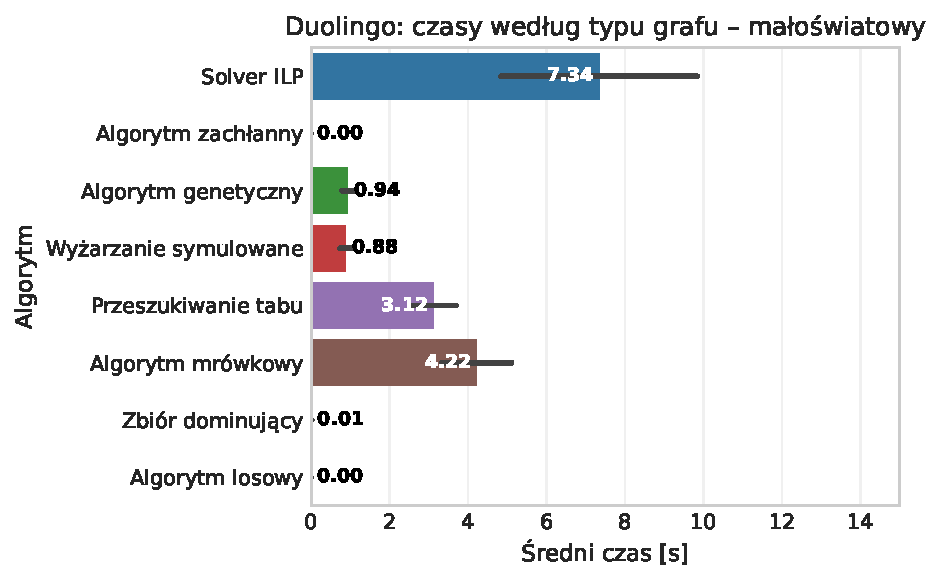
\includegraphics[width=0.65\linewidth]{assets/figures/benchmark/synthetic/duolingo_time_by_graph_small_world.pdf}
  \caption{Czas wykonania w zależności od struktury grafu małoświatowego.}
  \label{fig:duo-synth-time-small-world}
\end{figure}

\begin{table}[H]
  \centering
  \caption{Średnie koszty i czasy na węzeł dla różnych typów grafów (schematy licencyjne Duolingo Super i dominowania rzymskiego).}
  \label{tab:duo-synth-summary-times}
  \begin{tabular}{lcccc}
    \toprule
    \textbf{Licencja}    & \textbf{Typ grafu} & \textbf{Śr. koszt/węzeł} & \textbf{Śr. czas [s]} \\
    \midrule
    Duolingo Super       & Bezskalowy         & 0.661                    & 1.655                 \\
    Duolingo Super       & Losowy             & 0.502                    & 1.598                 \\
    Duolingo Super       & Małoświatowy       & 0.495                    & 1.346                 \\
    dominowanie rzymskie & Bezskalowy         & 0.490                    & 0.913                 \\
    dominowanie rzymskie & Losowy             & 0.344                    & 0.815                 \\
    dominowanie rzymskie & Małoświatowy       & 0.409                    & 1.544                 \\
    \bottomrule
  \end{tabular}
\end{table}

Z powyższych danych wynika, że schemat licencyjny dominowania rzymskiego osiąga niższy koszt na węzeł we wszystkich typach grafów syntetycznych. Największą przewagę wykazuje w grafach losowych (różnica 0{,}158), następnie w bezskalowych (0{,}171), a najmniejszą w małoświatowych (0{,}086). Pod względem czasów wykonania algorytmy dla schematu Duolingo Super charakteryzują się dłuższymi czasami w strukturach bezskalowych i losowych, jednak w grafach małoświatowych działają nieco szybciej niż w schemacie dominowania rzymskiego. Struktura bezskalowa generuje najwyższy koszt dla obu schematów licencjonowania, natomiast grafy małoświatowe zapewniają najkorzystniejszy stosunek kosztu do wydajności obliczeniowej. Przewaga kosztowa schematu dominowania rzymskiego wynika naturalnie z tego, że stosunek ceny licencji grupowej do indywidualnej jest w niej niższy niż w schemacie Duolingo Super.


\section{Duolingo Super na grafach rzeczywistych}
W analizie grafów ego z serwisu Facebook pominięto obserwacje, w których algorytm ILP nie zakończył pracy przed limitem czasu (18 przypadków). Dodatkowo odnotowano 8 przekroczeń limitu czasu algorytmu mrówkowego i 6 przypadków w przeszukiwaniu tabu; pozostałe uruchomienia zakończyły się sukcesem.

\begin{table}[H]
  \centering
  \caption{Statystyki kosztu i czasu dla schematu licencyjnego Duolingo Super na grafach rzeczywistych.}
  \label{tab:duo-real-alg}
  \begin{tabular}{lrrr}
    \toprule
    \textbf{Algorytm}     & \textbf{Średni koszt} & \textbf{Śr. koszt/węzeł} & \textbf{Śr. czas [s]} \\
    \midrule
    Algorytm mrówkowy     & 83.58                 & 0.506                    & 5.124                 \\
    Zbiór dominujący      & 119.97                & 0.542                    & 0.017                 \\
    Algorytm genetyczny   & 118.36                & 0.515                    & 1.222                 \\
    Algorytm zachłanny    & 121.94                & 0.548                    & 0.001                 \\
    Algorytm losowy       & 179.90                & 0.799                    & 0.001                 \\
    Wyżarzanie symulowane & 120.90                & 0.531                    & 0.975                 \\
    Przeszukiwanie tabu   & 117.80                & 0.500                    & 3.298                 \\
    \bottomrule
  \end{tabular}
\end{table}
Tabela~\ref{tab:duo-real-alg} wskazuje, że zarówno przeszukiwanie tabu, jak i algorytm mrówkowy zachowują przewagę kosztową nad heurystykami losowymi i zachłannymi, kosztem dłuższego czasu działania.

\subsection{Skalowanie i jakość}

Rysunek~\ref{fig:duo-real-size} ilustruje, że koszt na węzeł pozostaje względnie stabilny niezależnie od liczby wierzchołków, z niewielkimi wahaniami spowodowanymi różnicami między poszczególnymi instancjami grafów. Przeszukiwanie tabu utrzymuje najniższe wartości, a algorytm mrówkowy osiąga wartości zbliżone. Czasy działania wszystkich metod nie przekraczają kilku sekund i rosną łagodnie wraz z rozmiarem grafu; algorytm zachłanny zachowuje czas działania rzędu milisekund i stanowi efektywną procedurę inicjalizacji dla metaheurystyk. Dodatkowo tabela~\ref{tab:duo-real-size-table} agreguje średnie wartości (przeszukiwanie tabu) dla kolejnych rozmiarów sieci ego i pokazuje, że koszt na węzeł oscyluje w przedziale 0.37--0.56 przy czasie rosnącym od około 2~s do około 33~s dla największych grafów.

\begin{figure}[H]
  \centering
  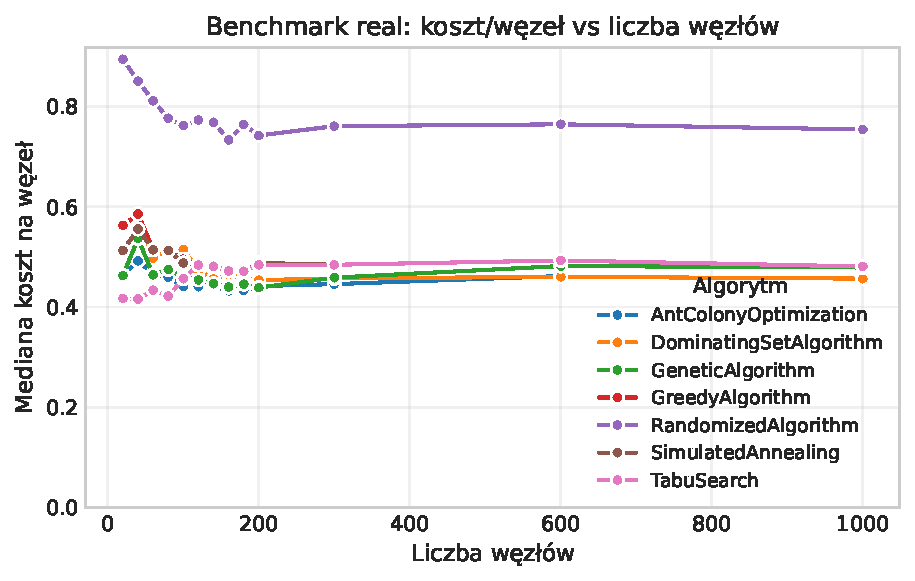
\includegraphics[width=0.48\linewidth]{assets/figures/benchmark/real/cost_per_node_vs_nodes.pdf}
  \hfill
  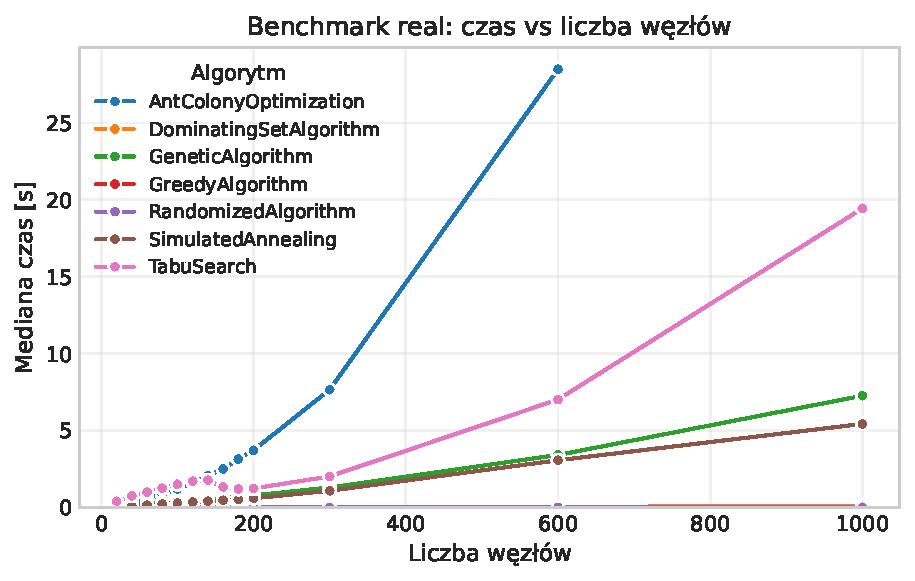
\includegraphics[width=0.48\linewidth]{assets/figures/benchmark/real/time_vs_nodes.pdf}
  \caption{Koszt na węzeł i czas wykonania algorytmów dla schematu licencyjnego Duolingo Super w zależności od liczby wierzchołków (grafy ego Facebook).}
  \label{fig:duo-real-size}
\end{figure}

\begin{table}[H]
  \centering
  \caption{Średni koszt licencji na węzeł i czas (przeszukiwanie tabu) względem liczby wierzchołków w sieciach ego Facebook.}
  \label{tab:duo-real-size-table}
  \begin{tabular}{lrr}
    \toprule
    \textbf{Liczba wierzchołków} & \textbf{Śr. koszt/węzeł} & \textbf{Śr. czas [s]} \\
    \midrule
    53                           & 0.441                    & 2.16                  \\
    62                           & 0.370                    & 3.14                  \\
    151                          & 0.379                    & 6.83                  \\
    169                          & 0.393                    & 8.73                  \\
    225                          & 0.408                    & 12.32                 \\
    334                          & 0.561                    & 32.71                 \\
    \bottomrule
  \end{tabular}
\end{table}


\section{Porównanie z dominowaniem rzymskim}

Porównania schematu licencyjnego Duolingo Super z konfiguracją imitującą dominowanie rzymskie ograniczono do wspólnych instancji grafów i algorytmów. Rysunki~\ref{fig:duo-roman-cost}--\ref{fig:duo-roman-license} zestawiają różnice w kosztach, czasach i strukturze licencji, a tabela~\ref{tab:duo-roman-graph} gromadzi średnie według typu grafu syntetycznego.

\begin{table}[H]
  \centering
  \caption{Średnie czasu i kosztu na węzeł według typu grafu (wspólne instancje).}
  \label{tab:duo-roman-graph}
  \begin{tabular}{lcccc}
    \toprule
    \multirow{2}{*}{\textbf{Typ grafu}} & \multicolumn{2}{c}{\textbf{Duolingo Super}} & \multicolumn{2}{c}{\textbf{dominowanie rzymskie}}                                            \\
                                        & \textbf{Czas [s]}                           & \textbf{Koszt/węzeł}                              & \textbf{Czas [s]} & \textbf{Koszt/węzeł} \\
    \midrule
    Losowy                              & 1.598                                       & 0.502                                             & 0.815             & 0.344                \\
    Bezskalowy                          & 1.655                                       & 0.661                                             & 0.913             & 0.490                \\
    Małoświatowy                        & 1.346                                       & 0.495                                             & 1.544             & 0.409                \\
    \bottomrule
  \end{tabular}
\end{table}

Algorytmy optymalizacji dla schematu licencyjnego dominowania rzymskiego osiągają niższy koszt na węzeł we wszystkich porównywanych typach grafów. Największa różnica dotyczy struktur losowych, gdzie przewaga wynosi ok.~0{,}158 jednostki kosztu na węzeł (32\%). W sieciach bezskalowych różnica wynosi 0{,}171 jednostki, natomiast w małoświatowych 0{,}086 jednostki. Algorytmy dla różnych schematów licencyjnych wykazują porównywalne czasy wykonania, przy czym w grafach małoświatowych algorytmy dla schematu licencyjnego Duolingo Super działają nieznacznie szybciej, natomiast w grafach losowych i bezskalowych szybciej działają algorytmy dla schematu licencyjnego dominowania rzymskiego. Rysunek~\ref{fig:duo-roman-cost} ilustruje te obserwacje dla pełnego rozkładu kosztów, a rysunek~\ref{fig:duo-roman-time} prezentuje analogiczne dane dotyczące czasów wykonania. Warto zauważyć, że wyższe koszty na węzeł w przypadku Duolingo Super wynikają z ograniczeń w opłacalności licencji grupowych. Licencja grupowa jest około 2{,}1 razy droższa od indywidualnej, co oznacza, że opłaca się ją tworzyć dopiero dla grup liczących co najmniej trzy osoby (właściciel i dwaj sąsiedzi w grafie). W konsekwencji liczba licencji indywidualnych w schemacie Duolingo Super jest większa, co przekłada się na wyższy średni koszt na węzeł w porównaniu z konfiguracją dominowania rzymskiego.

\begin{figure}[H]
  \centering
  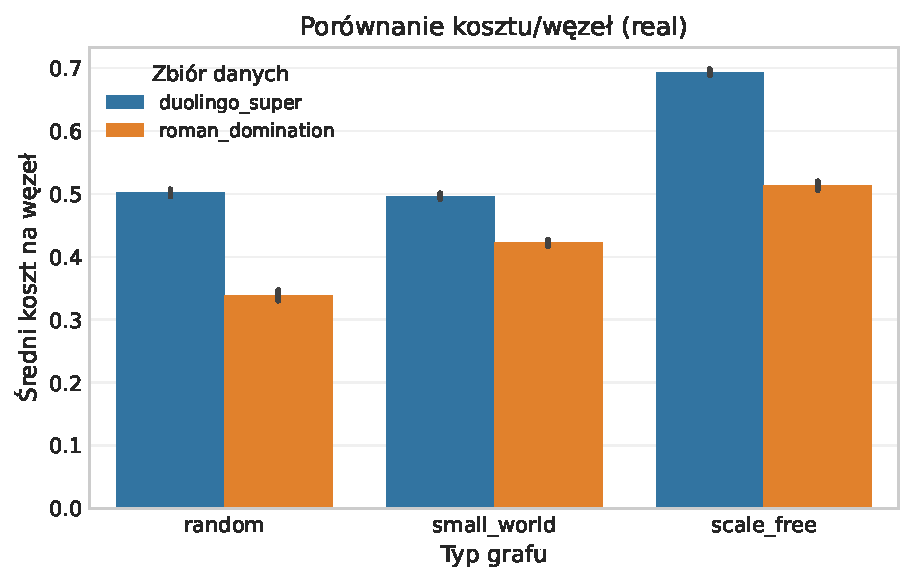
\includegraphics[width=0.6\linewidth]{assets/figures/benchmark/real/duo_vs_roman_cost_per_node_by_graph.pdf}
  \caption{Koszt na węzeł według typu grafu: porównanie konfiguracji licencyjnych Duolingo Super i dominowania rzymskiego.}
  \label{fig:duo-roman-cost}
\end{figure}

\begin{figure}[H]
  \centering
  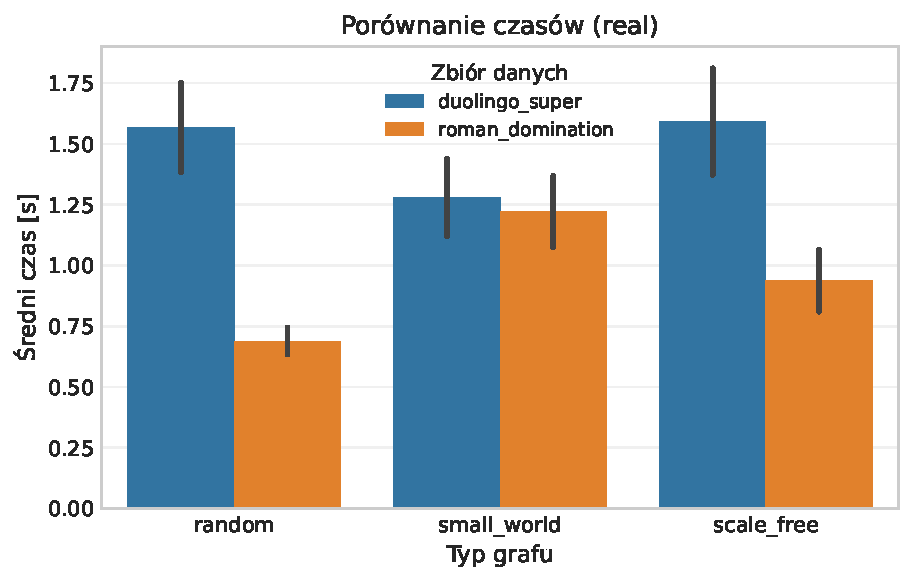
\includegraphics[width=0.6\linewidth]{assets/figures/benchmark/real/duo_vs_roman_time_by_graph.pdf}
  \caption{Czas wykonania według typu grafu: porównanie konfiguracji licencyjnych Duolingo Super i dominowania rzymskiego.}
  \label{fig:duo-roman-time}
\end{figure}

Rysunek~\ref{fig:duo-roman-license} pokazuje, że w rozwiązaniach optymalnych dla konfiguracji licencyjnej dominowania rzymskiego obserwuje się wyższy stosunek licencji grupowych do indywidualnych w porównaniu do rozwiązań dla konfiguracji licencyjnej Duolingo Super. W konfiguracji dominowania rzymskiego stosunek licencji grupowych do indywidualnych wynosi około 1{,}15:1, natomiast w schemacie Duolingo Super stosunek ten jest odwrócony i wynosi około 0{,}88:1 (więcej licencji indywidualnych niż grupowych).

Różnica w strukturze wykorzystania licencji wynika z faktu, że konfiguracja licencyjna dominowania rzymskiego nie posiada ograniczenia maksymalnej pojemności grupy licencyjnej. W schemacie Duolingo Super, gdy grupa osiąga maksymalną pojemność, dodatkowi użytkownicy, którzy mogliby do niej należeć, są zmuszeni do zakupu licencji indywidualnych. W pełnym zbiorze danych, obejmującym trzy typy grafów syntetycznych, odnotowano 137 690 licencji w schemacie Duolingo Super, z czego 73 176 (53{,}15\%) to licencje indywidualne. W konfiguracji dominowania rzymskiego, dzięki brakowi ograniczeń pojemności grup, liczba licencji indywidualnych jest proporcjonalnie niższa.

\begin{figure}[H]
  \centering
  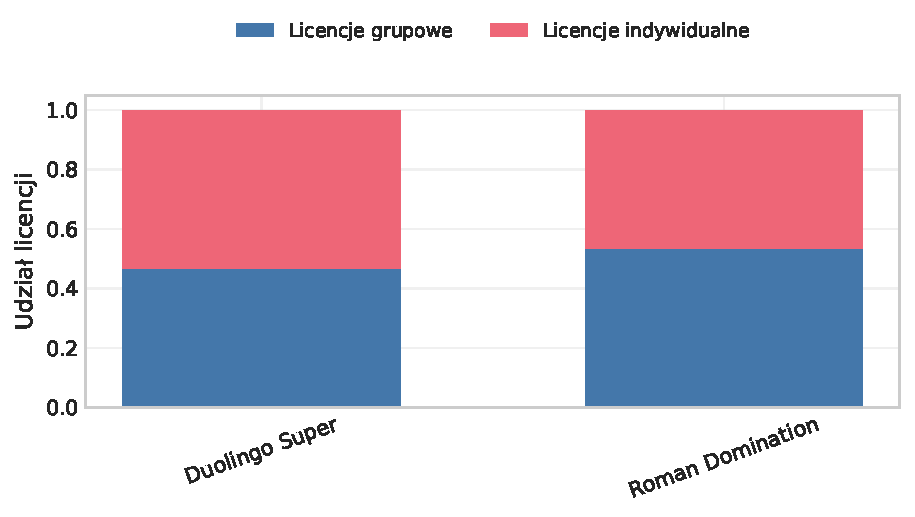
\includegraphics[width=0.6\linewidth]{assets/figures/benchmark/synthetic/license_mix_duo_vs_roman.pdf}
  \caption{Struktura wykorzystania licencji: porównanie konfiguracji licencyjnych Duolingo Super i dominowania rzymskiego.}
  \label{fig:duo-roman-license}
\end{figure}

\section{Wnioski}

Przeprowadzone eksperymenty wskazują, że schemat licencjonowania Duolingo Super zapewnia stabilne i powtarzalne wyniki. Spośród badanych metod najlepsze wyniki uzyskały algorytm mrówkowy oraz przeszukiwanie tabu. Algorytm mrówkowy osiąga najniższy koszt na węzeł w grupie metaheurystyk, lecz wymaga dłuższego czasu działania. Przeszukiwanie tabu umożliwia uzyskanie porównywalnej jakości i jednocześnie zachowuje lepszy kompromis między kosztem a czasem obliczeń.

Solver ILP stanowi wartościowe odniesienie jakościowe, jednak jego zastosowanie jest ograniczone do mniejszych instancji ze względu na częste przekroczenia limitu czasu. Proste heurystyki, takie jak algorytm zachłanny czy losowy, charakteryzują się bardzo krótkim czasem działania, ale rozwiązania mają istotnie wyższy koszt na węzeł.

Wyniki potwierdzają również znaczenie struktury grafu. W przypadku grafów losowych i małoświatowych możliwe jest osiągnięcie rezultatów zbliżonych do solvera ILP, natomiast grafy bezskalowe okazały się trudniejsze i generowały wyższe koszty. Skalowanie pokazane na rysunku~\ref{fig:duo-real-size} dowodzi, że przeszukiwanie tabu zachowuje niskie koszty na węzeł nawet przy rosnącej liczbie wierzchołków, a czasy działania rosną umiarkowanie.

Porównanie ze schematem licencyjnym dominowania rzymskiego wskazuje, że schemat ten osiąga niższy koszt na węzeł we wszystkich typach grafów. Wynika to z większego udziału licencji grupowych i niższego kosztu jednostkowego. Schemat Duolingo Super cechuje się natomiast krótszym czasem wykonania w grafach małoświatowych.
